\documentclass[12pt, a4paper]{report}

\usepackage{fyp}

%%these packages are not really necessary if you dont need the code and proofs environments
%%so if you like you can delete from here till the next comment
%%note that there are some examples below which obviously won't work once you remove this part
\usepackage{verbatim}
\usepackage{amsfonts}
\usepackage{amsmath}
\usepackage{amssymb}
\usepackage{amsthm}
\usepackage{natbib}
\usepackage{url}

%%this environment is useful if you have code snippets
\newenvironment{code}
{\footnotesize\verbatim}{\endverbatim\normalfont}

%%the following environments are useful to present proofs in your thesis
\theoremstyle{definition}
\newtheorem{definition}{Definition}[section]
\theoremstyle{definition}%plain}
\newtheorem{example}{Example}[section]
\theoremstyle{definition}%remark}
\newtheorem{proposition}{Proposition}[section]
\theoremstyle{definition}%remark}
\newtheorem{lemma}{Lemma}[section]
\theoremstyle{definition}%remark}
\newtheorem{corollary}{Corollary}[section]
\theoremstyle{definition}%remark}
\newtheorem{theorem}{Theorem}[section]
%%you can delete till here if you dont need the code and proofs environments



\setlength{\headheight}{15pt}
%\overfullrule=15pt


\begin{document}



%%make sure to enter this information
\title{Adapting Pretrained Models for Machine Translation}
\author{Aditya Kurniawan}
\date{enter a date}
\supervisor{Marc Tanti}
\department{Faculty of ICT}
\universitycrestpath{img/crest}
\submitdate{enter a date}

\frontmatter


\begin{acknowledgements}
    your acknowledgments
\end{acknowledgements}

\begin{abstract}
    an abstract an abstract an abstract an abstract an abstract an abstract an abstract an abstract an abstract an abstract an abstract an abstract an abstract an abstract an abstract an abstract an abstract an abstract an abstract an abstract an abstract an abstract an abstract an abstract an abstract an abstract an abstract an abstract an abstract an abstract an abstract an abstract an abstract an abstract an abstract an abstract an abstract an abstract an abstract an abstract an abstract an abstract an abstract an abstract an abstract an abstract an abstract an abstract an abstract an abstract an abstract an abstract an abstract an abstract an abstract an abstract an abstract an abstract an abstract an abstract an abstract an abstract an abstract an abstract an abstract an abstract an abstract an abstract an abstract an abstract an abstract an abstract an abstract an abstract an abstract an abstract an abstract an abstract an abstract an abstract an abstract an abstract an abstract an abstract an abstract an abstract an abstract an abstract an abstract an abstract an abstract an abstract an abstract an abstract an abstract an abstract an abstract
\end{abstract}

\tableofcontents

\listoffigures

\listoftables



\mainmatter

% \chapter{Introduction}
% Lorem ipsum dolor sit amet, id mel movet dicit accusamus, eam te assum liber. Te ferri habemus his. Eum te cibo noster, et illud etiam est, mei detraxit democritum in. Ei ius audiam sanctus. Eu has nobis cetero, ea est modus mazim, at eam magna tantas delenit. Ad mucius fabulas percipit quo.

% Sea nostrum scribentur ex, in eam reque incorrupte, te quis audiam antiopam mei. Id audiam option oportere eum, esse brute ut eos. Sea ubique legere cu, eum ne quas decore expetendis. Aeque fierent mnesarchum cum te, vix verterem iudicabit ea.
\chapter*{Introduction}
\addcontentsline{toc}{chapter}{Introduction}
Pre-trained language models \citewithpar{devlin2018bert,howard2018universal} have received considerable attention in recent years. These models are trained on large-scale corpora and then fine-tuned for a particular downstream task. This method allows pre-trained models to perform well across various natural language processing tasks. One of the most successful models is BERT \citewithpar{devlin2018bert}. BERT has been most extensively used for common natural language understanding (NLU) tasks. It has been shown that BERT can achieve great performance with relatively straightforward fine-tuning, especially for classification-like tasks.

For natural language generation (NLG), incorporating BERT is still challenging. According to \normcite{zhu2020incorporating}, simply incorporating BERT into the encoder side of the seq2seq architecture can hurt the performance. On the decoder side, BERT does not quite fit either because the bidirectional nature of the model was significantly different from the objective of the conditional language model (predicting the next word).

Fine-tuning all BERT's parameters is inefficient, given that there are approximately 200 million parameters in a single model of BERT. Naive fine-tuning also often results in catastrophic forgetting, where the models forget the previous knowledge they have acquired while improving on the new domain \citewithpar{mccloskey1989catastrophic,yogatama2019learning}. This may explain why it is considered harmful to simply fine-tune an initialized encoder component with BERT. It is also known that fine-tuning large pre-trained language models could result in unstable and fragile performance on small datasets.

Adapter is an alternative approach that allows for fine-tuning a model without altering the original network weights \citewithpar{houlsby2019parameter,bapna2019simple}. By leveraging adapters, one can reduce the number of parameters updated in fine-tuning and make the process computationally less expensive while achieving similar results. Another useful property of the approach with adapters is that they are more robust against catastrophic forgetting than fine-tuning \citewithpar{han2021robust}.

This work uses BERT and its variants as the base pre-trained models and fine-tune them with adapters. We evaluate the models on machine translation with the following objectives:
\begin{itemize}
    \item We conduct a study to understand the contribution of good representation in the pre-trained language model when fine-tuning using adapters.
    \item We conduct a study to evaluate the effectiveness of adapters in the seq2seq framework by putting them only in the encoder or the decoder.
    \item We experiment with down-scaling the pre-trained model size and try to recover the performance from being comparable to the full-sized model.
\end{itemize}

\section*{Thesis Organization}

\paragraph{Chapter 1} discusses the theoretical background of machine translation, transfer learning, and a brief overview of the current state of using adapters in various setups.

\paragraph{Chapter 2} reviews the previous related work on transfer learning from models that were pre-trained on language model objectives and the usage of adapters in various disciplines within text and speech domains.

\paragraph{Chapter 3} describes the dataset that we use to train language models and machine translation. We then explain the pre-processing of the dataset and the tokenization to construct the vocabularies. Finally, we describe the framework for the experiments and the automatic evaluation metric.

\paragraph{Chapter 4} presents our attempt to use adapters in machine translation setup. This chapter focuses on the contribution of pre-trained representations when fine-tuning with adapters. We discuss the result of our experiments by referring to the automatic evaluation metric as well as providing our own manual analysis. Furthermore, we discuss the limitation of incorporating BERT in machine translation by providing the translation output errors.

\paragraph{Chapter 5} presents our attempt to understand the effectiveness of adapters and the impact of the pre-trained weights for adapters by placing them only in the encoder or decoder. We then continue the experiments by down-scaling BERT to half of the size and trying to recover the adapter's performance so that it is comparable to the full-sized model. We provide discussions of the phenomenon that happens when reducing the size of the original BERT model.

\paragraph{Conclusion} summarizes our findings from the experiments.


\section{Section name}

Duo commodo copiosae ne, nec ei novum meliore constituto, cu mea duis tamquam. Docendi elaboraret in has, hinc principes ex sit. Option inermis elaboraret an sea. Ne sed dicunt salutandi deterruisset, eum alia quas voluptatibus ei.

No vim tempor mediocritatem necessitatibus. Mea doming maluisset eu, no pro omnes meliore, ne pri odio purto recusabo. Te duo solet facete feugiat, nullam virtute intellegat vix ea. Exerci posidonium in usu. Meis omittam aliquando cum ea, ius feugait detraxit deseruisse eu. At mel viderer virtute contentiones, et eos omnis senserit euripidis.


%%you can organise your chapters into parts but this is not always necessary
%%\part{Part1} - Available but generally not used
% \chapter{Chapter name}

% Sea no ullum euripidis scriptorem, ne aperiam voluptaria qui, quo eros lobortis quaerendum in. No velit recteque cum. Posse semper complectitur vel et, has intellegat instructior ei. Decore doming quo in, an eum duis patrioque. Eu nam choro vituperata, et qui quas porro epicurei. Pro an aliquando intellegat inciderint, quo munere civibus an.
\chapter{Title of the first chapter}

An~example citation: \cite{Andel07}
This is to modify

\section{Title of the first subchapter of the first chapter}

\section{Title of the second subchapter of the first chapter}

\chapter{Title of the second chapter}

\section{Title of the first subchapter of the second chapter}

\section{Title of the second subchapter of the second chapter}

% Target 5 pages

\chapter{Experiment Setup}
\label{chap:03}
In this chapter, we describe our selection of datasets, framework, and automatic evaluation we used for the experiments. We start by describing our set of training and test data, our reasoning for choosing the dataset, and the tokenization algorithm in \cref{sec:dataset}. We then move forward to the framework we use to implement the neural network, training, and evaluation phase in \cref{sec:framework}. Finally, we discuss the automatic evaluation we use during the experiments in  \cref{sec:aeval}.

\section{German-to-English Dataset}
\label{sec:dataset}
The scope of our experiment is in a single language pair: German$\rightarrow$English. We only select a single language pair because we want to focus our experiment on understanding the behaviour of BERT and the adapters in machine translation, not on generalization across multiple language pairs. We select IWSLT14 and WMT19 as our primary datasets. IWSLT14 will be mainly used as the dataset for fine-tuning and testing the final performance of the model, while WMT19 is used for the additional dataset in pre-training as well as in training some of our baselines.

\subsection{IWSLT 2014}
The 2014 IWSLT evaluation \citewithpar{Cettolo2014ReportOT} is the fourth instance of a shared task started in 2010. This task is mainly focusing on the translation of TED Talks. The task is based on a collection of public speeches that cover various topics. All the talks in the collections have English captions. These captions are then translated into many languages by various volunteers worldwide. As TED talks are recorded events of speakers sharing their thoughts and experience, we need to deal with spoken language rather than written language. Spoken language is expected to be less complex and formal than written language.

Both the in-domain training and development data are available through the WIT3 website.\footnote{\url{https://wit3.fbk.eu/}} There is also out-of-domain training data provided through the workshop website. We focus only on the English German pairs in this work and ignore the other available languages. The evaluation dataset (tst2014) comprises talks from the previous years, and the 2014 talks are included in the training sets. Furthermore, to improve the reliability of assessing the MT progress over the years, evaluation sets from previous years (tst2013) are also distributed together with tst2014. On the other hand, development sets (dev2010, tst2010, tst2011, and tst2012) are kept intact from the past editions.

Evaluation sets tst2014 for the German language (De$\rightarrow$En) are derived from the ASR task. Therefore, it is ensured that no overlap exists with other tasks that employ TED talks. In addition to the TED talks, there is a series of independent talks called TEDx. The difference lies in the location of the events. TED talks mainly focus on the North American region, while TEDx can be held in various areas worldwide. The TEDx-based corpus was proposed in 2013 for De$\rightarrow$En as an additional test set to put more rigour into the evaluation process. Finally, a concatenation of the TEDx and TED-based development sets consisting of dev2010, tst2010, tst2011 and tst2012 sets were released. The complete statistics of the dataset can be seen in \cref{tab:iwslt14stat}.

\begin{table}[h]
    \centering
    \begin{tabular}{@{}cclll@{}}
        \toprule
        \multicolumn{2}{c}{\multirow{2}{*}{\textbf{set}}} & \multicolumn{1}{c}{\multirow{2}{*}{\textbf{sentences}}} & \multicolumn{2}{c}{\textbf{tokens}}                                           \\ %\cmidrule(l){4-5}
        \multicolumn{2}{c}{}                              & \multicolumn{1}{c}{}                                    & \multicolumn{1}{c}{\textbf{En}}     & \multicolumn{1}{c}{\textbf{De}}         \\ \toprule
        \multicolumn{2}{c}{train}                         & 172k                                                    & 3.46M                               & 3.24M                                   \\ \midrule
        \multirow{4}{*}{dev}                              & TED.dev2010                                             & 887                                 & 20,1k                           & 19,1k \\
                                                          & TED.tst2010                                             & 1,565                               & 32,0k                           & 30,3k \\
                                                          & TED.tst2011                                             & 1,433                               & 26,9k                           & 26,3k \\
                                                          & TED.tst2012                                             & 1,700                               & 30,7k                           & 29,2k \\ \midrule
        \multirow{5}{*}{test}                             & TED.tst2013                                             & 993                                 & 20,9k                           & 19,7k \\
                                                          & TED.tst2014                                             & 1,305                               & 24,8k                           & 23,8k \\
                                                          & TEDx.dev2012                                            & 1,165                               & 21,6k                           & 20,8k \\
                                                          & TEDx.tst2013                                            & 1,363                               & 23,3k                           & 22,4k \\
                                                          & TEDx.tst2014                                            & 1,414                               & 28,1k                           & 27,6k \\ \bottomrule
    \end{tabular}
    \caption{Statistics of IWSLT 2014 German$\rightarrow$English dataset.}
    \label{tab:iwslt14stat}
\end{table}

\subsection{WMT 2019}
WMT19 dataset was first introduced in The Fourth Conference on Machine Translation (WMT) held at ACL 2019 \citewithpar{barrault-etal-2019-findings}. The primary objectives of this conference are to evaluate the state-of-the-art models in MT, advertise public access to the MT models' performance and the common test sets, and improve the methods to evaluate and estimate machine translation. There are various shared tasks within the conference that evaluate different machine translation aspects. This conference has been conducted 13 times and the current conference is built on top of the previous editions \citewithpar{koehn-monz-2006-manual,callison-burch-etal-2007-meta,callison-burch-etal-2008-meta,callison-burch-etal-2009-findings,callison-burch-etal-2010-findings,callison-burch-etal-2011-findings,callison-burch-etal-2012-findings,bojar-etal-2013-findings,bojar-etal-2014-findings,bojar-etal-2015-findings,bojar-etal-2016-findings,bojar-etal-2017-findings,bojar-etal-2018-findings}.

The dataset was collected from various news sources on the Internet. As mentioned before, we use WMT for the pre-training dataset and an additional dataset to train our baseline models. For this reason, we are not utilizing the dev and test set. Therefore, we show the statistics of the dataset in \cref{tab:wmt19stat} only for the training set. Apart from a large number of sentences, another reason for choosing WMT19 as our additional dataset is that it contains sentence pairs from various domains.

\begin{table}[h]
    \centering
    \begin{tabular}{@{}llll@{}}
        \toprule
        \multicolumn{1}{c}{\multirow{2}{*}{\textbf{corpus}}} &
        \multicolumn{1}{c}{\multirow{2}{*}{\textbf{sent}}}   &
        \multicolumn{2}{c}{\textbf{tokens}}                                            \\
        \multicolumn{1}{c}{}                                 &
        \multicolumn{1}{c}{}                                 &
        \multicolumn{1}{c}{\textbf{De}}                      &
        \multicolumn{1}{c}{\textbf{En}}                                                \\ \midrule
        Europarl Parallel Corpus                             & 1,8M  & 48,1M  & 50,5M  \\
        News Commentary Parallel Corpus                      & 0,3M  & 8,3M   & 8,2M   \\
        Common Crawl Parallel Corpus                         & 2,3M  & 54,5M  & 58,8M  \\
        ParaCrawl Parallel Corpus                            & 31,3M & 559,3M & 598,3M \\
        EU Press Release Parallel Corpus                     & 1,4M  & 29,4M  & 30M    \\
        WikiTitles Parallel Corpus                           & 1,3M  & 2,8M   & 3,2M   \\ \bottomrule
    \end{tabular}
    \caption{Statistics of WMT 2019 German$\rightarrow$English dataset.}
    \label{tab:wmt19stat}
\end{table}

\subsection{Tokenization}
% - Using huggingface implementation of WordPiece https://huggingface.co/docs/transformers/tokenizer_summary
BERT uses the subword tokenization algorithm called WordPiece \citewithpar{schuster2012japanese} to construct the list of vocabularies. The algorithm is very similar to Byte-Pair Encoding (BPE; \cite{sennrich-etal-2016-neural}), where it relies on a pre-tokenizer to split words within the training data, such as simple whitespace tokenization.

After the pre-tokenization, the set of words with their frequency is gathered. BPE then starts building a symbol vocabulary that consists of all symbols within the corpus. The symbol can be anything from alphabetical, numeric, and other symbols. BPE then learns a set of rules to merge and form a new symbol from two other symbols from the existing vocabulary. This process is repeated until the size of vocabulary items matches the desired vocabulary size.

To provide an example, let us assume that we have the following words and their frequencies\footnote{The example is taken from \url{https://huggingface.co/docs/transformers/tokenizer_summary}}:

\bigskip
("hug", 10), ("pug", 5), ("pun", 12), ("bun", 4), ("hugs", 5)
\bigskip

From these words, we have the set of initial symbols: ``["b", "u", "n", "p", "h", "g", "s"]''. BPE then starts the merging process by using the total frequency of each possible symbol pair. The pair that occurs the most often will be picked as a new vocabulary item. In our example, we have "h" followed by "u" with a total of 15 occurrences (10 times in \texttt{hug} and 5 times in \texttt{hugs}) and "u" followed by "g" with a total of 20 occurrences. Therefore, we pick "ug" and append the new symbol to the vocabulary. We repeat this process until we meet the desired number of vocabulary items.

During the decoding process and assuming the following set of unique symbols: ``["b", "u", "n", "p", "h", "g", "s", "ug"]'', we now perform the tokenization process by matching the sub-word of the input word to the existing vocabulary. For example, if the incoming word is "mug", we will have ["[UNK]", "ug"] as our tokenization as we do not have "m" in our vocabulary. "[UNK]" is introduced as a special symbol to handle tokens/symbols that do not exist in the vocabulary. On the other hand, the word "bug" will be tokenized into ["b", "ug"].

\section{Framework}
\label{sec:framework}
\subsection{HuggingFace Transformers}
Transformers \citewithpar{wolf2020transformers} is a library created by the Huggingface team that implements various transformer-based architectures. This library's primary aim is to implement transformer models specifically designed for research and production. This implies that the library is easy to read, extend, and supported by the industrial-strength implementation for deployment in production. The library also aims to facilitate transformer-based pre-trained model distribution to the public. Under the same foundation, this library supports the distribution and re-use of various pre-trained models in a centralized hub. This includes the configuration, such as the hyperparameters used to instantiate the models and the pre-trained weights. This improves research reproducibility as numerous users can now re-use and improve their experiments based on the pre-trained models.

The fact that the library is continuously maintained by the Huggingface team and supported by over 400 external contributors is one of our reasons for choosing Huggingface to conduct the experiments in this work. The library is released under the Apache 2.0 license and is freely available on GitHub and their official website.\footnote{\url{https://github.com/huggingface/} and \url{https://huggingface.co}} Furthermore, the website also provides easy-to-understand tutorials and detailed documentation of the API.

\subsection{AdapterHub}
Another reason we choose Huggingface is the availability of AdapterHub \citewithpar{pfeiffer-etal-2020-adapterhub}. Despite adapter's simplicity and achieving strong results in multi-task and cross-lingual transfer learning \citewithpar{pfeiffer2021adapterfusion,pfeiffer2020madx}, reusing and sharing adapters was not straightforward. Adapters are rarely released independently due to their subtle differences in architecture and strong dependence on the base model, task, and language. AdapterHub was created to facilitate the easiness of training models with adapters and share the fine-tuned adapters in various settings to mitigate these issues.

\section{Automatic Evaluation}
\label{sec:aeval}
Bilingual Evaluation Understudy or \texttt{BLEU} \citewithpar{BLEU} is one of the evaluation metrics that is widely used to evaluate MT models. It works by evaluating the output of an MT system (the hypothesis) with a set of manually translated references.

BLEU works by measuring the percentage of the matching n-grams in the hypothesis and taking the difference in length of the hypothesis and references as a form of penalty. The percentage of n-grams is often interpreted as a measurement of precision. However, in some cases, simply calculating the matching n-grams may lead to a misinterpretation of the output. In the case of unigram ($n=1$), we can see the matching n-grams as the number of tokens available in the hypothesis and the references divided by the total number of tokens. See the following example:

\bigskip

\textbf{Hypothesis}: \underline{you} \underline{you} \underline{you} \underline{you}

\textbf{Reference}: I think \underline{you} should know that \underline{you} are right

\bigskip

The above example will lead to 100\% unigram precision of the hypothesis despite the result only sharing the word \textbf{you}. To mitigate the precision problem, the shared number of n-grams in the hypothesis and the reference must be clipped by the number of n-grams in the reference. The following is the updated BLEU formula after incorporating the n-gram clipping:

\begin{equation}
    p_n=\frac{\sum_{C\in\{Candidates\}}\sum_{n\in C}Count_{clip}(n)}{\sum_{C'\in\{Candidates\}}\sum_{n'\in C'}Count(n')}
\end{equation}

Where $n$ is the set of possible n-grams from a particular sentence used when calculating the score.

We mentioned that besides n-grams, BLEU also considers the length of the hypothesis as a penalty score. This is useful when dealing with short candidates within the hypothesis. The following is the example that shows the problematic output:

\bigskip

\textbf{Hypothesis}: you

\textbf{Reference}: I think \underline{you} should know that \underline{you} are right

\bigskip

Despite having a 100\% precision score, the hypothesis does not represent the correct translation compared to the reference. We want to elude such a problem by introducing a penalty called \textbf{brevity penalty}. The penalty works by measuring the length of the hypothesis relative to the reference length and  $e^{(1-r/c)}$ when the candidate is shorter than the reference length. To be more specific, we refer to the equation below.

\begin{equation}
    BP=\begin{cases} 1 & \mbox{if } c>r \\ e^{(1-r/c)} & \mbox{if } c\le r \end{cases}
\end{equation}

In the case of more than one reference, $r$ is the length of the reference with the closest length to the hypothesis, called the \textbf{effective reference length}. One must note that the choice of reference will vary between different implementations of BLEU. To be more precise, take the following example that shows the difference between two references is equal to 1, where one reference is one word shorter than the hypothesis and the other is one word longer:

\bigskip

\textbf{Candidate}: I eat fish on the beach with

\textbf{Reference} 1: I eat fish on the beach with friends

\textbf{Reference} 2: I eat fish on the beach

\bigskip

Combining the above components, BLEU is defined as follows:

\begin{equation}
    BLEU=BP\cdot exp\left( \sum_{n=1}^{N} w_n \log p_n \right)
\end{equation}

We define $w_n$ as the weights for each n-grams scores ($p_n$) where $\sum^{\infty}_{i=1} w_i = 1$. $w_n$ is usually set uniformly across all $n$ depending on the number of n-grams used in the calculation. When 4-grams is used, it is set to $\frac{1}{4}$.

By default, BLEU computes the n-gram precision from unigrams to 4-grams. We perform the final score computation by calculating the average for each n-gram score and multiplying them by the brevity penalty (BP).

In this work, we follow the implementation of sacrebleu\footnote{\url{https://github.com/mjpost/sacreBLEU}} \citewithpar{post-2018-call} that is wrapped under Huggingface Transformers framework.
\chapter{Experiments Results}

\section{Adapters Comparison}
\begin{figure}[h]
    {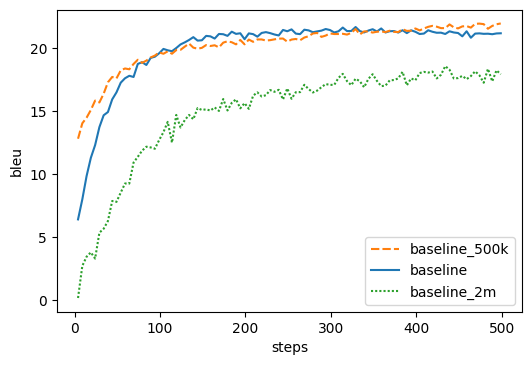
\includegraphics[width=0.95\textwidth]{img/baseline.png}}
    \centering
    \caption{
        Comparison between baseline models trained with different size of datasets. \texttt{baseline} represents the model trained only using IWSLT; \texttt{baseline\_500k} represents the model trained using IWSLT and WMT with total of 500k sentence pairs; \texttt{baseline\_2m} represents the model trained using IWSLT and WMT with total of 2 million sentence pairs.}
    \label{img:basecomp}
\end{figure}

In this section, we compare the result of the baseline models with the models that are fine-tuned with adapters. From Figure \ref{img:basecomp}, adding more data to the baseline models does not necessarily improve the performance. We suspect the models require more time to train to get better performance. There is a clear gap between \texttt{baseline\_2m} and the rest of the baseline models. \texttt{baseline} and \texttt{baseline\_500k} performs really well from the start while \texttt{baseline\_2m} lag behind. We suspect this is the effect of including more sentences from different domains. \texttt{baseline\_500k} is the best mix given the training time constraint. It provides a balance in between not overfitting in the correct domain and not too much data out of the domain. \texttt{baseline\_2m} shows the impact on domain difference. It does not perform well on IWSLT but it is growing and has a chance to improve the performance further. At a later stage, the \texttt{baseline\_2m} output would deserve manual evaluation, because the lower bleu may not necessarily reflect a lower quality, we can see some of the result in Table \ref{tab:qtvout}.

To see the impact of including adapters, we compare the result on different sizes of pre-training used for the base model. The base models are then fine-tuned with the adapters module on the IWSLT data. As we can see from Figure \ref{img:adpcomp}, BERT achieves the best performance from the earlier steps compared to the rest of the pre-training size. In contrast to the baseline models, we see the benefit of adding more sentences to the pre-training. We can see the performance progression between the model that was trained using 500k data has lower performance than the one using 2 million data. On the other hand, models that only use IWSLT as the pre-training data suffers from performance degradation in the middle of the fine-tuning. We observed that this is due to the gradient explosion on the cross-attention layer. The IWSLT model eventually managed to achieve a similar performance to the 500k model in the later steps.
\begin{figure}[h]
    {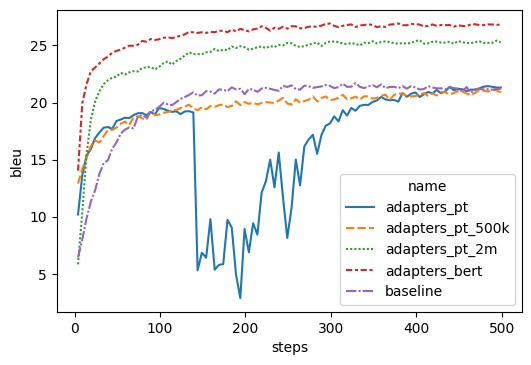
\includegraphics[width=0.95\textwidth]{img/adapterscomparison.png}}
    \centering
    \caption{
        % \XXX{Could you include baseline curve, too? This is rather important for comparison given the lack of the stopping criterion.}
        Comparison between adapters pre-trained with different size of datasets. \texttt{baseline} represents the model trained only using IWSLT; \texttt{adapters\_pt} represents the model pre-trained only using IWSLT; \texttt{adapters\_pt\_500k} represents the model pre-trained using IWSLT and WMT with total of 500k sentence pairs; \texttt{adapters\_pt\_2m} represents the model pre-trained using IWSLT and WMT with total of 2 million sentence pairs; \texttt{adapters\_bert} represents the model that uses BERT weights.}
    \label{img:adpcomp}
\end{figure}

\begin{table*}[]
    \centering
    \begin{tabular}{l}
        \hline
        \multicolumn{1}{c}{\textbf{Random Weights + Adapters}} \\ \hline
        \begin{tabular}[c]{@{}l@{}}\textbf{input}: wir tanzen im tempel und werden zu gott. \& quot ;\\ \textbf{prediction}:we \& apos ; re going to be able to become god. \& quot ;\end{tabular}                              \\ \hline
        \begin{tabular}[c]{@{}l@{}}\textbf{input}: aber gleichzeitig hatten sie eine klare kenntnis des waldes, die erstaunlich war.\\ \textbf{prediction}:but at the same time, they had a clear of the audience who was amazing..\end{tabular}                              \\ \hline
        \begin{tabular}[c]{@{}l@{}}\textbf{input}: es ist so wunderbar. ihr musst es beschutzen. \& quot ;\\ \textbf{prediction}:it \& apos ; s wonderful. you have to protect it. \& quot ;\end{tabular}                              \\ \hline
    \end{tabular}
    \caption{Prediction results from randomly set pre-trained model fine-tuned with adapters}
    \label{tab:qtrand}
\end{table*}

\section{Random and Shuffled Pre-training Weights}
We can see from Figure \ref{img:shfrndcmp} that the performance of the model that uses random weights as the pre-training model is more stable than the one using shuffled BERT weights. Both of the shuffled BERT models suffer from gradient explosion similar to the IWSLT model we show in the previous section. Although the performance of the random model is still below the baseline model, it is interesting to see that only fine-tuning adapters and the cross-attention layer manage to achieve a reasonable BLEU score, considering that the pre-training models do not contain any meaningful information.
\begin{figure}[h]
    {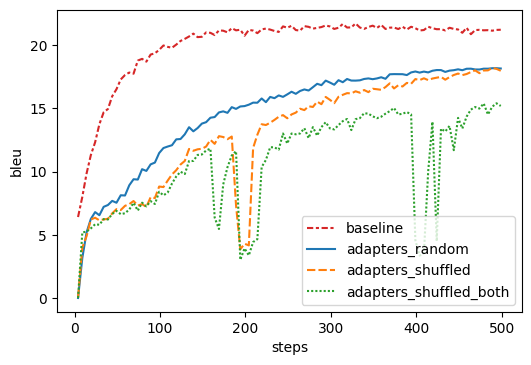
\includegraphics[width=0.95\textwidth]{img/randomshuffled.png}}
    \centering
    \caption{Comparison between adapters using shuffled BERT and random weights as the pre-trained models. \texttt{baseline} represents the model trained only using IWSLT; \texttt{adapters\_random} represents the model pre-trained only using random weights; \texttt{adapters\_shuffled} represents the model pre-trained using column-wise shuffled BERT model; \texttt{adapters\_shuffled\_both} represents the model pre-trained using shuffled BERT model.}
    \label{img:shfrndcmp}
\end{figure}

\section{Random Pretraining vs. Out-of-Domain Data}
We further analyze the random weights by comparing the result with the best performing, baseline, and transformer models we pre-trained ourselves. From Figure \ref{img:rndbslcmp}, we can see that the performance of the random model achieves a similar result to the baseline model that uses 2 million training sentence pairs. While the performance is still far from the baseline that is trained using only IWSLT data, this result shows the base model's structure helps the adapter achieve a meaningful performance with very small weights required for the fine-tuning.

We perform a quick check to the output of the model in Table \ref{tab:qtrand}. We can see from the first two lines that the model hash difficulty to capture complex phrases. On the first row, the model missed \textbf{tanzen im tempel} which means \textbf{dancing in the temple}. For the second row, the model confuses \textbf{knowledge of the forest} and output \textbf{audience instead}. Furthermore, the model also does not translate the word \textbf{kenntnis} and makes the translation unclear since the object of the sentence is missing. Despite those mistakes, the model still can capture simple sentences as shown on the third row. Another observation that we noticed in the generated output is the tokenization of \texttt{\&quot\;} and \texttt{\&amp\;}. Instead of being treated as a single token, the tokenizer treats the token as three different subword token. We notice that this is due to the inavailability of the aforementioned token in the pre-trained BERT vocabulary.


\begin{figure}[h]
    {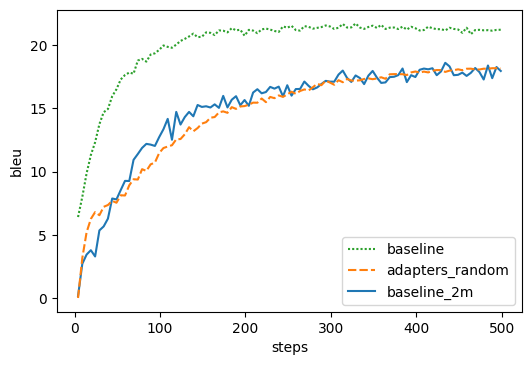
\includegraphics[width=0.95\textwidth]{img/random.png}}
    \centering
    \caption{Comparison between pre-trained random weights and baseline model. \texttt{baseline} represents the model trained only using IWSLT; \texttt{baseline\_2m} represents the baseline model trained with a combination of IWSLT and WMT sentence pairs; \texttt{adapters\_random} represents the model pre-trained only using random weights; \texttt{adapters\_pt\_2m} represents the model pre-trained using IWSLT and WMT with total of 2 million sentence pairs; \texttt{adapters\_bert} represents the model that uses BERT weights}
    \label{img:rndbslcmp}
\end{figure}

\section{Qualitative Comparison}
\begin{table*}[]
    \begin{tabular}{|l|l|l|}
        \hline
        \multicolumn{1}{|c|}{\textbf{Baseline IWSLT}}        &
        \multicolumn{1}{c|}{\textbf{IWSLT + WMT (total 2m)}} &
        \multicolumn{1}{c|}{\textbf{BERT + Adapters}}          \\ \hline
        \begin{tabular}[c]{@{}l@{}}\textbf{input}: erinnerst du dich an\\ den patienten\\ mit dem gereizten rachen? \\ \textbf{prediction}: do you remember\\ reading to the patients? on the\end{tabular}                            &
        \begin{tabular}[c]{@{}l@{}}\textbf{input}: erinnerst du dich an\\ den patienten\\ mit dem gereizten rachen? \\ \textbf{prediction}: do you remember\\ the patient with the tingling\\ revenge?\end{tabular}                            &
        \begin{tabular}[c]{@{}l@{}}\textbf{input}: erinnerst du dich an\\ den patienten\\ mit dem gereizten rachen? \\ \textbf{prediction}: remember the\\ patient with\\ the bruised remorse?\end{tabular}                             \\ \hline
        \begin{tabular}[c]{@{}l@{}}\textbf{input}: großartig, sagte ich.\\ legte auf.\\ \textbf{prediction}: great, i said.\\ got up..\end{tabular}                           &
        \begin{tabular}[c]{@{}l@{}}\textbf{input}: großartig, sagte ich.\\ legte auf.\\ \textbf{prediction}: great, i said.\\ put on..\end{tabular}                           &
        \begin{tabular}[c]{@{}l@{}}\textbf{input}: großartig, sagte ich.\\ legte auf.\\ \textbf{prediction}: great, i said.\\ put it down.\end{tabular}                             \\ \hline
        \begin{tabular}[c]{@{}l@{}}\textbf{input}: - - aber in unserer\\ entdeckung der welt, haben\\ wir alle arten unterschiedlicher\\ methoden.\\ \textbf{prediction}: but in our discovery\\ of the world, we \& apos ;\\ ve got all sorts of different\end{tabular}                           &
        \begin{tabular}[c]{@{}l@{}}\textbf{input}: - - aber in unserer\\ entdeckung der welt, haben\\ wir alle arten unterschiedlicher\\ methoden.\\ \textbf{prediction}: - - but in our discovery\\ of the world, we have\\ all kinds of different methods.\end{tabular}                           &
        \begin{tabular}[c]{@{}l@{}}\textbf{input}: - - aber in unserer\\ entdeckung der welt, haben\\ wir alle arten unterschiedlicher\\ methoden.\\ \textbf{prediction}: but in our discovery\\ of the world, we have\\ all sorts of different ways of doing\\ things.\end{tabular}                             \\ \hline
    \end{tabular}
    \caption{Prediction results from 1) Baseline model trained with only IWSLT data; 2) Pre-trained model with adapters where we pre-train the model with IWSLT and WMT with a total of 2 million pre-training data; 3) BERT with adapters.}
    \label{tab:qtvout}
\end{table*}
We perform a sanity check to compare the generated results on some of our models. This sanity check is to check the errors produced by the models on different techniques.
From Table \ref{tab:qtvout}, we can see for the first example none of the models managed to generate the correct result. However, BERT + adapters and 2 million pre-trained base models manage to generate the proper context where the result is still discussing \textbf{the patient}. The wrong part is when the model generates an incorrect translation regarding the patient's disease. The second example shows that the BERT + adapters create the correct and better output than the other models. The final example shows that BERT + adapters generate an interesting output where it manages to remove unimportant characters such as \texttt{--} and produce readable output. There may be a slightly different opinion on this example as the 2 million pre-trained base model generate a more concise output.


% \section{Section name}

% Section content

% \section{Section name}

% Section content

% \begin{definition}
%     This is an example of a definition
% \end{definition}

% \begin{example}
%     This is an example of an example :)
% \end{example}


% \chapter{Chapter Name}

% \section{Section Name}

% \begin{proof}
%     this is a proof
% \end{proof}


% \chapter{Conclusion}
\chapter*{Conclusion}
\addcontentsline{toc}{chapter}{Conclusion}



\appendix

\chapter{This chapter is in the appendix}
\section{These are some details}
%%example of the code environment
\begin{code}
    this is some code;
    Make sure to use this template.
\end{code}


\bibliomatter



\bibliographystyle{abbrv}
\bibliography{bibliography}

\end{document}
